%! TEX root = ../000-main.tex
\chapter{Observed functional data and its computational representation}
\chaptermark{Observed FD}

\section{Observing functional data in practice}

It is not possible to observe (sample) and/or to record (store)
a functional data $\mathcal X_i$ for all $t\in T=[a,\,b]$:
\begin{itemize}
	\item The measurement devices are only able to sample the phenomenon
	      only at discrete instants (even if the sample frequency is extremely high).
	\item Given that $T = [a,\,b]$ is an infinite set, saving all
	      $\mathcal X_i$ for all $t\in T$ would imply to use an infinite amount of memory.
\end{itemize}

In practice, $\mathcal X_i$ is sampled/recorded in a finite grid:
\begin{equation*}
	t_{i1} < \cdots < t_{im_i} \subset T
\end{equation*}
where $m_i$ is the number of samples. If $m_i$ is large enough,
the maximum difference between two consecutive samples
$\max_j\left\{t_{ij} - t_{i(j+1)}\right\}$ is small.

This presents 4 scenarios, as depicted in \cref{fig:observed-fd-scenarios}:
\begin{figure}[H]
	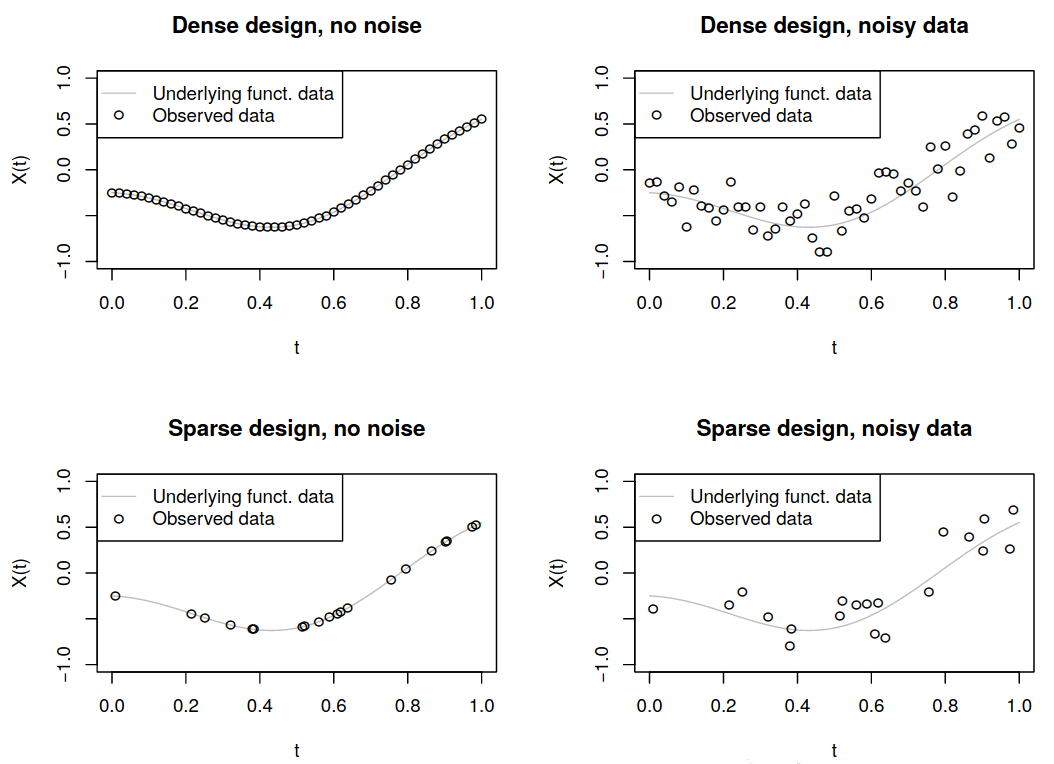
\includegraphics{observed-fd-scenarios}
	\caption{Example scenarios for the observation of functional data}
	\label{fig:observed-fd-scenarios}
\end{figure}

\subsection{Dense design}

\begin{definition}{Evenly Spaced Sampling}{}
	\begin{equation*}
		t_{j+1} - t_j = \delta = \frac{t_m - t_1}{m}
	\end{equation*}
\end{definition}

\subsection{Sparse design}

% TODO

\begin{definition}{Functional Data (practical definition)}{fdp}
	Multivariate data with an ordering on the dimensions.

	This definition implicitly assumes a common ordered design:
	\begin{equation*}
		t_1 < \cdots < t_m :  \mathcal X_i (t_j) + \varepsilon_{ij},\quad
		j=1,\ldots,m,\quad i=1,\ldots,n
	\end{equation*}
	\tcblower
	\begin{note}
		Ordering in the $m$ dimensions of the data is \emph{curcial},
		because it allows us to talk about \iemph{close dimensions}%
		\footnote{Close dimensions are more correlated than \iemph{distant dimensions}.}%
		.
	\end{note}
	\begin{note}
		This is an alternative way of saying that the functional data
		$\mathcal X_i$ are smooth functions.
	\end{note}
\end{definition}

\begin{question*}
	{Is FDA really different from Multivariate Analysis?}
	\begin{itemize}
		\item In Functional Data Analysis, the methods and procedures are
		      designed as if the functional data $\mathcal X_i(t),\,t\in T=[a,\,b]$
		      were available.
		\item Then the observed data $x_{ij}$ are used to estimate the required
		      elements.
		\item Finally, the outputs are displayed taking into account the functional
		      character of the objects of interest.
	\end{itemize}
\end{question*}



\pagebreak
\section[Representing functional data]{Representing functional data in a computer}

\subsection{Matrix representation}

\subsubsection{Common evenly spaced dense design}
Common evenly spaced (or not) dense design with no noisy data:
\begin{equation*}
    x_{ij} = \mathcal X_i(t_j),\quad j=1,\ldots,m,\quad i=1,\ldots,n
\end{equation*}
already have a good representation as a $n\times m$ matrix
$\boldsymbol X = \left(x_{ij}\right)_{n\times m}$.

If $\delta = t_{j+1} - t_j$ is small enough, many (if not all) the
required methods and procedures in FDA can be satisfactorily numerically
approximated using this matrix representation.

\subsubsection{Other situations}
For functional data with noisy data and/or sparse design, \iemph{smoothing
methods} allows us to obtain a smooth estimation of the
underlying functional data with a common evenly spaced dense design. This
estimations can then be represented as a matrix.

\subsection{Basis-expansion representation}

Consider the square integrable Hilbert Space $L^2(T)$.
The inner product $\langle f, g\rangle = \int_T f(t)g(t)\,dt$ induces
a norm $\|f\| = \sqrt{\langle f, f\rangle}$ and a distance
between two functions $d(f, g)$:
\begin{equation*}
    d(f, g) = \lVert f - g \rVert = \sqrt{\langle f - g, f - g\rangle}
\end{equation*}

\begin{prop*}{}
    Any separable Hilbert space admits a countable orthonormal basis.
\end{prop*}

\begin{definition}{Countable Orthonormal basis}{}
    A countable family $B = \{\phi_k\}_{k\in\mathds N},\,\phi_k\in H$ of functions
    that satisfies:
    \begin{alignat*}{2}
        \langle \phi_k, \phi_j\rangle &= 0, \quad &\forall& k,j \in \mathds N, k\neq j
        \tag{orthogonality} \\
        \lVert \phi_k \rVert &= 1 \quad& \forall& k \in \mathds N \tag{Normalization} \\
        \tag{Completeness}
    \end{alignat*}
\end{definition}

\subsubsection{Finite basis}

\subsubsection{Fourier basis}


% \section{Developments in bases of functions}
% \section{Smoothing: Kernel, Local Polynomials, Splines}
% \section{Registration and transformations of functional data}
